\scanpage{5}
\mspage{2}
(ce qui est sans doute tjrs vrai, et \deleted{dans} le critère d'une non sauvagerie de $\gamma$) on est ramené au cas précédent, en \deleted{enlevant} remplaçant $Y'$ par $Y'\setminus S'$, où $S'$ est l'ens. fini des pts de ramification pour l'action de $\gamma$. \deleted{\unsure{$E$}}

On fera attention que la \deleted{condition} \inserted{propriété} envisagée \deleted{n'est pas} (sur les autom. d'ordre fini de la surface $Y'$) n'est pas vérifiée sans restriction. Si p.ex. $Y'=\mathbb{C}^*$, ou $Y'=\mathbb{U}\times\mathbb{U}$ alors les translations par des points d'ordre fini sont isotopes à l'identité, sans être néc. égaux à l'identité ! Mais on a ceci
\figure{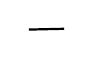
\begin{tikzpicture}[baseline=0pt]\draw[line width=.8pt] (0,0)--(.45,.01);\end{tikzpicture}}

\uline{Proposition 2} Soit $Y'$ une surface orientée de t.f. (\inserted{surf.} cpte $-$ nb fini de pts) \uline{anabélienne}, i.e. telle que pour tte comp. connexe $Y'_i$ de $Y'$, on ait $\chi_!(Y'_i)<0$ (i.e. on ait $2g_i+\nu_i\geq 3$, où $g_i$ est le genre de $Y'_i$ et $\nu_i$ le nb des trous\ldots). Alors tout autom. \inserted{$\gamma$} d'ordre fini de $Y'_i$ qui est isotope à l'identité est l'identité.

Comme $\gamma$ invarie les composantes connexes, OPS $Y'$ connexe. En fait, il suffit que $\gamma$ opère trivialement sur la homologie \inserted{$H_1$} (\inserted{p.ex.} à coefficients dans $\mathbb{Z}$, ou dans \inserted{un} $\mathbb{Z}/n\mathbb{Z}$ avec $n\geq3$) pour
\margin{4}
